\chapter{Presentation of Software}

\begin{longtabu}{rX}
    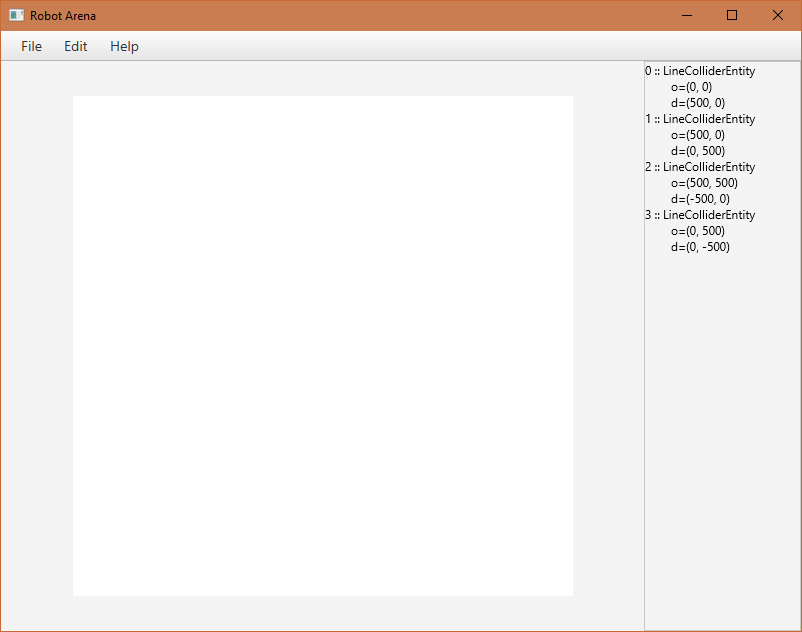
\includegraphics[width=0.4\linewidth,valign=t]{img/01.png} & The stock interface of the software shows the stock interface. The top menu bar provides all functionality of the software, the white square in the middle represents the environment scaled onto a square canvas, the text to the right specifies entities in the arena and their statistics. The four entities in the arena by default when opened are the walls of the arena at it's boundaries. \\
    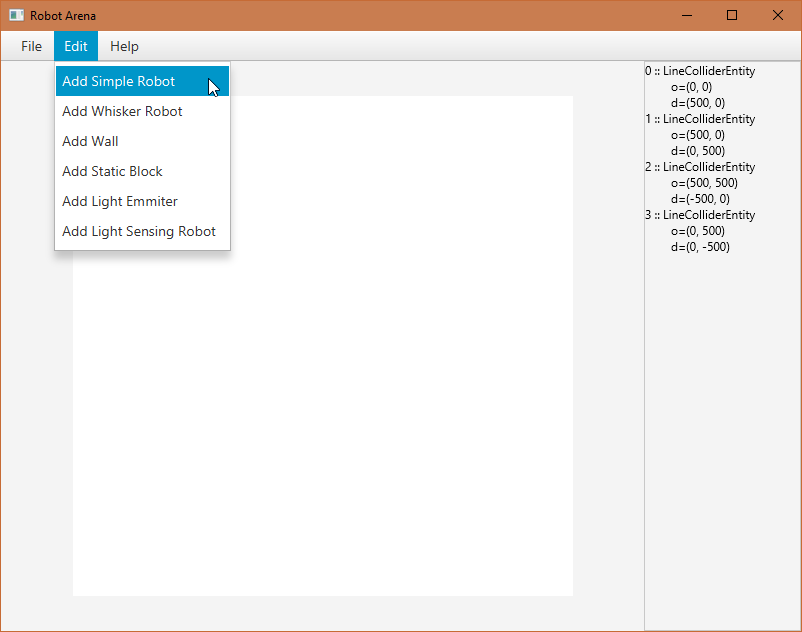
\includegraphics[width=0.4\linewidth,valign=t]{img/02.png} & The edit interface allows you to add a variety of randomly initialised entities, including robots, lights, and obstacles to the arena. \\
    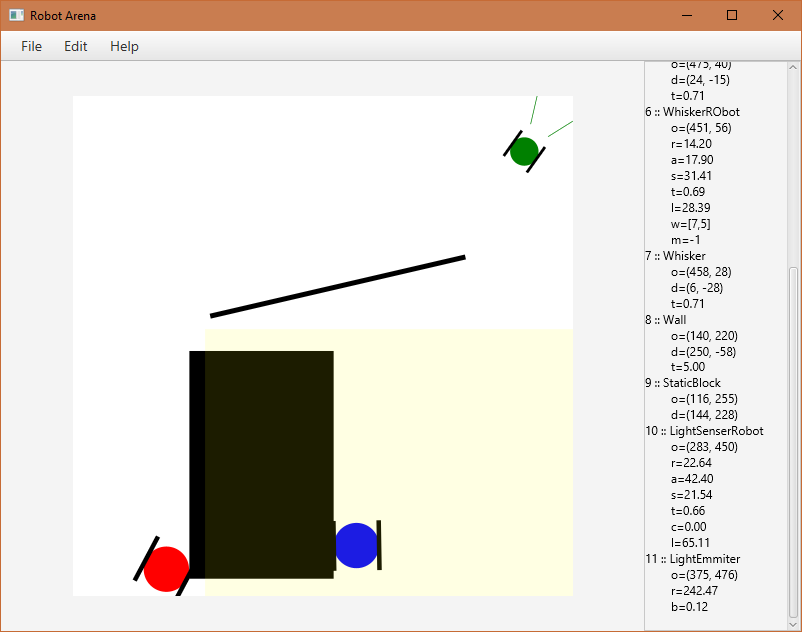
\includegraphics[width=0.4\linewidth,valign=t]{img/03.png} & Arena after one of each of the options from the edit menu is clicked. \\
    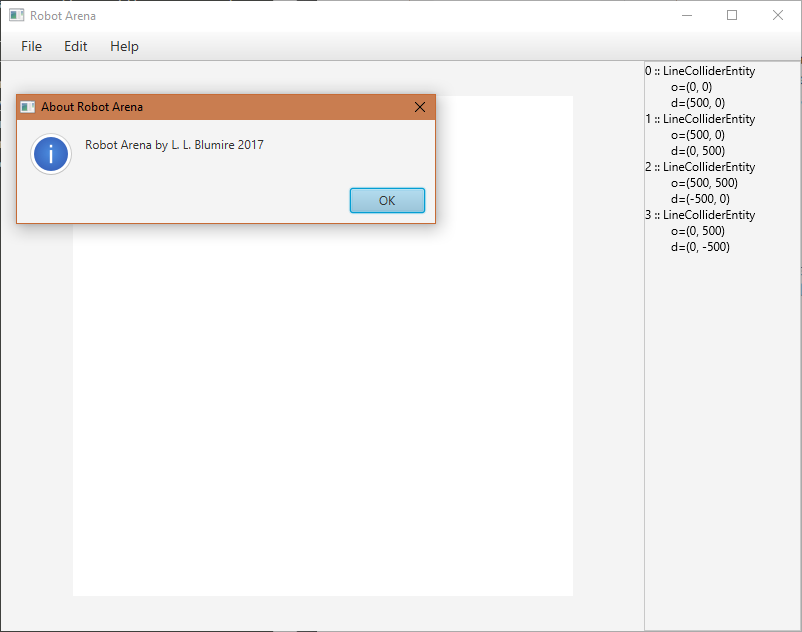
\includegraphics[width=0.4\linewidth,valign=t]{img/04.png} & The dialog that appears when selecting `About' in the `Help' menu. \\
    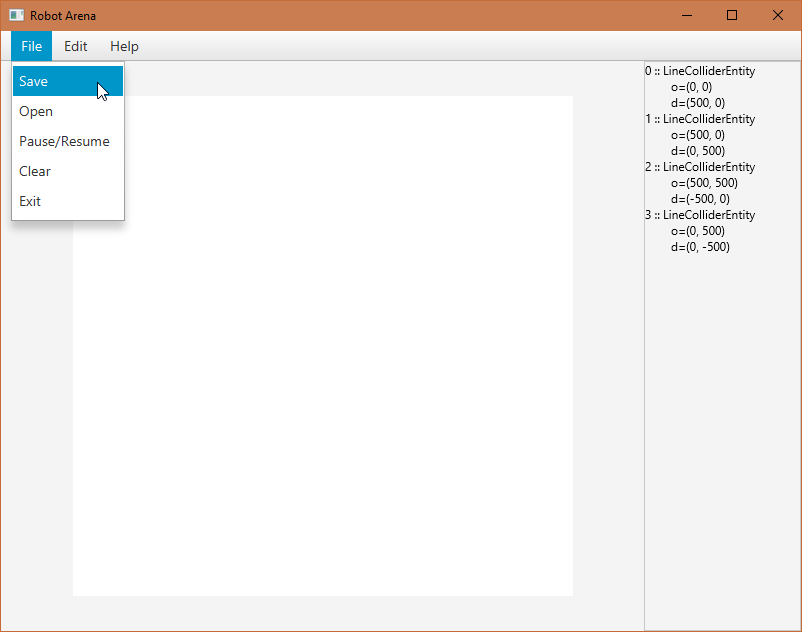
\includegraphics[width=0.4\linewidth,valign=t]{img/05.png} & The contents of the File menu, includes clearing and re-initialising the arena, saving and loading the arena to a file, pausing and resuming the simulation of the arena, and exiting the program. \\
    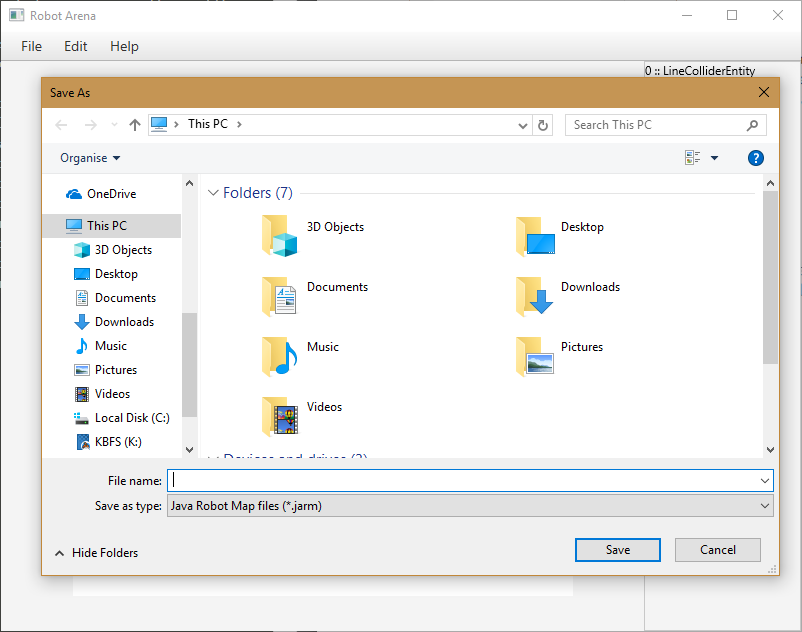
\includegraphics[width=0.4\linewidth,valign=t]{img/06.png} & The result of clicking on the save option, load option functions similarly.
\end{longtabu}